\problemname{Logic Circuit}

Here is a simple logic circuit that has $3$ inputs, $A$, $B$, and $C$, and $1$ output $D$.

\begin{figure}[ht!]
  \centering
    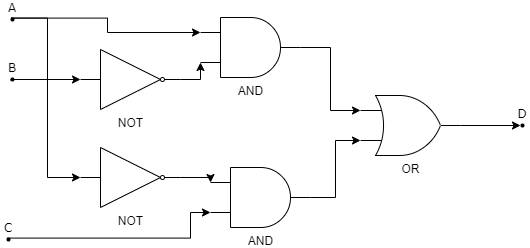
\includegraphics[width=0.5\textwidth]{circuit}
  \caption{The logic circuit}
\end{figure}

The circuit contains three types of logic gates:

\begin{itemize}
    \item A \texttt{NOT} gate takes one input $x$, and outputs $1$ if $x=0$, but $0$ otherwise.
    \item An \texttt{AND} gate takes two inputs $x$ and $y$, and outputs $1$ if $x=y=1$, but $0$ otherwise.
    \item An \texttt{OR} gate takes two inputs $x$ and $y$, and outputs $0$ if $x=y=0$, but $1$ otherwise.
\end{itemize}

Write a program that is equivalent to the logic circuit above.

\section*{Input}
Input consists of three lines.
The first line contains the integer $A$, where $A$ is either $0$ or $1$.
The second line contains the integer $B$, where $B$ is either $0$ or $1$.
The third line contains the integer $C$, where $C$ is either $0$ or $1$.

\section*{Output}
Output the value of $D$, which is either $0$ or $1$.
